\section{Methoden}
	
	Dieser Abschnitt befasst sich mit dem Aufbau des Versuches und den dabei auftretenden Unsicherheiten.
	
	\subsection{Aufbau und Funktionsweise}	
		
		Der Versuchsaufbau besteht im Wesentlichen aus einem Stirling-Motor, ein mit dem Motor verbundenes Kühlwasserreservoir und einem Messgerät für die Rotation des Motors sowie der Temperatur des Wassers, welches sich in einem Reagenzglas an dem verschraubbaren Zylinderkopf des Stirling-Motors befindet.
		Das Messgerät ist an einen Computer geschlossen, sodass bei der Messung der Rotation zeitgleich ein FFT angewendet werden kann, um den Motor auf \SI{3}{\hertz} zu kalibrieren.
		Zur Messung der Temperatur des abfließenden Kühlwassers, bzw. der im Reservoir wird ein einfaches Digital-Thermometer verwendet.
		
		Abb. \ref{fig:Aufbau} stellt die Funktionsweise des Stirling-Motors schematisch dar. 
		Hierbei handelt es sich um einen Kreisprozess aus zwei isothermen und zwei isochoren Zustandsänderungen.
		Je nachdem in welche Richtung das Schwungrad (bzw. der Motor) dreht, wird der Stirling-Motor zur Kältemaschine (entgegen des Uhrzeigersinn) oder zur Wärmepumpe (im Uhrzeigersinn). 
		\begin{figure}[ht]
			\centering
			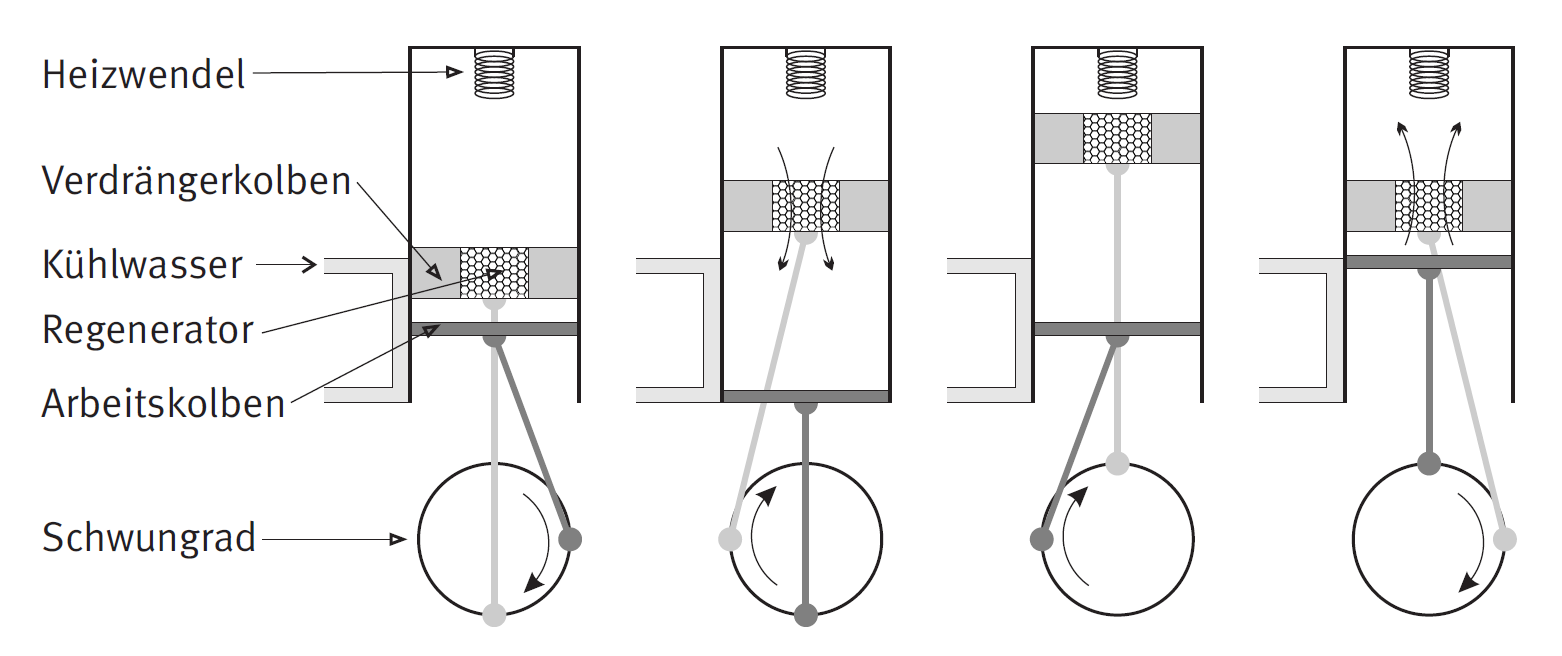
\includegraphics[width=\textwidth]{Aufbau.png}
			\caption{Darstellung der Takte des Stirling-Motors. Isotherme Expansion, isochore Abkühlung, isothemre Kompression und isochore Erwärmung (von links nach rechts).\cite{WWU}}
			\label{fig:Aufbau}	
		\end{figure}
				
	\subsection{Unsicherheiten}
	
		Jegliche Unsicherheiten werden nach GUM bestimmt und berechnet\footnote{Die Gleichungen dazu finden sich im Anhang unter \ref{fig:GUM_combine}, \ref{fig:GUM_formula}.}.
		Für die Unsicherheitsrechnungen wurde die Python Bibliothek "uncertainties" herangezogen, welche den Richtlinien des GUM folgt.
	
		Für digitale Messungen wird eine Unsicherheit von $u(X) = \frac{\Delta X}{\sqrt{3}}$ angenommen, bei analogen eine von $u(X) = \frac{\Delta X}{\sqrt{6}}$.
		
		\begin{description}
			\item[Abtastrate] Für die zeitliche Abtastrate des Messprogramms wurde eine Unsicherheit entsprechend der Abtastfrequenz mit $\Delta t = \frac{1}{f}$ gewählt.
			Die Messung erfolgt digital.
			
			\item[Position] Bei der Positionsbestimmung wurde durch die Schrittweite der Daten eine Unsicherheit von $\Delta x = \SI{0.1}{\milli\meter}$ festgelegt.
			Die Messung ist digital.
			
			\item[Stopuhr] Die Unsicherheit setzt sich aus der analogen Reaktionszeit und der digitalen Stellengenauigkeit nach \ref{fig:GUM_combine} zusammen.
			Die Zeit kann beim Messprozess gut abgeschätzt werden, da der Füllstand des Messzylinder linear zunimmt, also ist die Reaktionszeit auf $\Delta t_1 = \SI{0.1}{\second}$ abgeschätzt.
			Die Stopuhr kann zwei Nachkommastellen angeben, also ist $\Delta t_2 = \SI{10}{\milli\second}$.
			
			\item[Messzylinder] Das Volumen des Zylinders ist in \SI{1}{\milli\liter} unterteilt.
			Es wird analog abgelesen.
			Also folgt $\Delta V = \SI{1}{\milli\liter}$.
			
			\item[Pipette] Die Pipette, mit welcher die Probemenge bestimmt wurde, hatte auf \SI{1}{\milli\liter} Einhundert Unterteilungen und wurde ebenfalls analog abgelesen.
			Dementsprechend folgt $\Delta V = \SI{0.01}{\milli\liter}$.
			
			\item[Thermometer] Sowohl das Programm, als auch das manuelle Thermometer konnten auf eine Nachkommastelle genaue Angaben machen.
			Beide sind digital.
			Es ergibt sich die Unsicherheit $\Delta T = \SI{0.1}{\celsius}$.
		\end{description}
		
		In Diagrammen mit vielen Messpunkten wurden aus Gründen der Übersichtlichkeit nicht für jeden Punkt Unsicherheitsbalken gezeichnet.
		
\section{Durchführung und Datenanalyse}	
	\begin{figure}[ht]
		\centering
		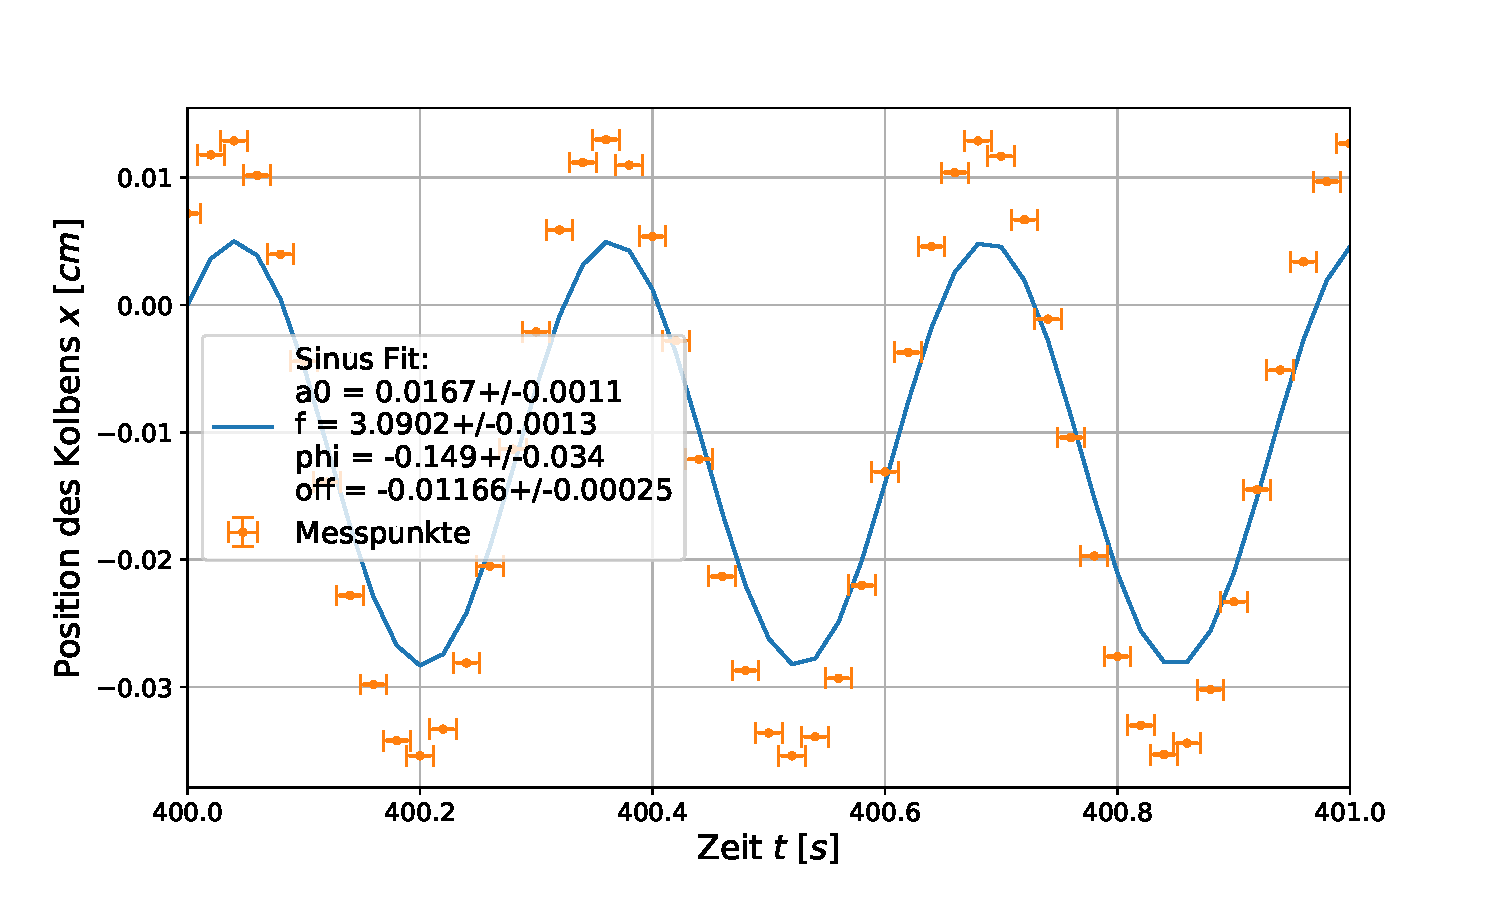
\includegraphics[width=\textwidth]{data/Position.pdf}
		\caption{Sinus-Fit zur Rotation des Motors.}
		\label{fig:Frequenz}	
	\end{figure}
	Damit der Motor mit einer Frequenz von $\approx$ \SI{3}{\hertz} arbeiten konnte, wurde seine Rotation aufgenommen und das Zeitbild am Computer fourier-transformiert, sodass eine passende Frequenz über Geschwindigkeitsänderung des Motors festgelegt werden konnte.
	Diese Messung ist in Abb. \ref{fig:Frequenz} mit einem Sinus-Fit dargestellt.
	Daraus folgte eine Frequenz von ca. \SI{3,09}{\hertz}, welche für die weiteren Berechnungen verwendet wurden.
	
	Zur Bestimmung der Reibungsarbeit wurde zunächst der Zylinderkopf des Stirling-Motors abgenommen und die Temperatur $T_0 = \SI{24,5+-0,03}{\celsius}$ des Kühlwassers an diesem gemessen.
	Dann  wurde der Motor als Wärmepumpe in Betrieb genommen.
	Ab dem Punkt, an dem die Temperatur des Kühlwassers sich nicht mehr änderte, bei $T_{max} = \SI{25,0+-0,03}{\celsius}$, wurde der Volumendurchfluss an dem Kühlwasserreservoir gemessen.
	Daraus ergab sich eine Zeit $t_{MB} = \SI{11,47+-0,003}{\second}$ für $V_{MB} = \SI{50+-0,2}{\milli\liter}$.
	Der Volumendurchfluss ergibt sich aus:
	\begin{equation} % massenstrom des Kühlwassers [masse pro zeit]
		M = \rho \frac{V_\text{MB}}{t_\text{MB}}.
	\end{equation} % rho ist dichte, V ist volumen des Messbechers, t ist Füllzeit des volumens
	Dabei ist $\rho$ die Dichte des Wassers.
	Allgemein gilt für das System:
	\begin{equation} % absolute Leistung der Maschine, ist dW < 0 so wird Energie aufgenommen, ist dW > 0 so wird Energie abgegeben/Arbeit von der Maschine geleistet; da wir hier Wärmepumpe/Kältemaschine haben ist dW < 0 und der Motor gibt Energie in das System ein
		W = Q_1 - Q_2 + W_\text{R},
	\end{equation} % Q_1 ist Wärme des Kühlwassers(negativ)[siehe (3)], Q_2 ist Wärme der Probe/gemessene Temperatur (4) -> Wärmeänderung(Kältemaschine: positiv, Wärmepumpe: negativ)
	wobei $W_\text{R}$ der gesuchten Reibungsarbeit entspricht.
	%TODO Rechenweg ↓ Reibung
	
	\begin{figure}[ht]
		\centering
		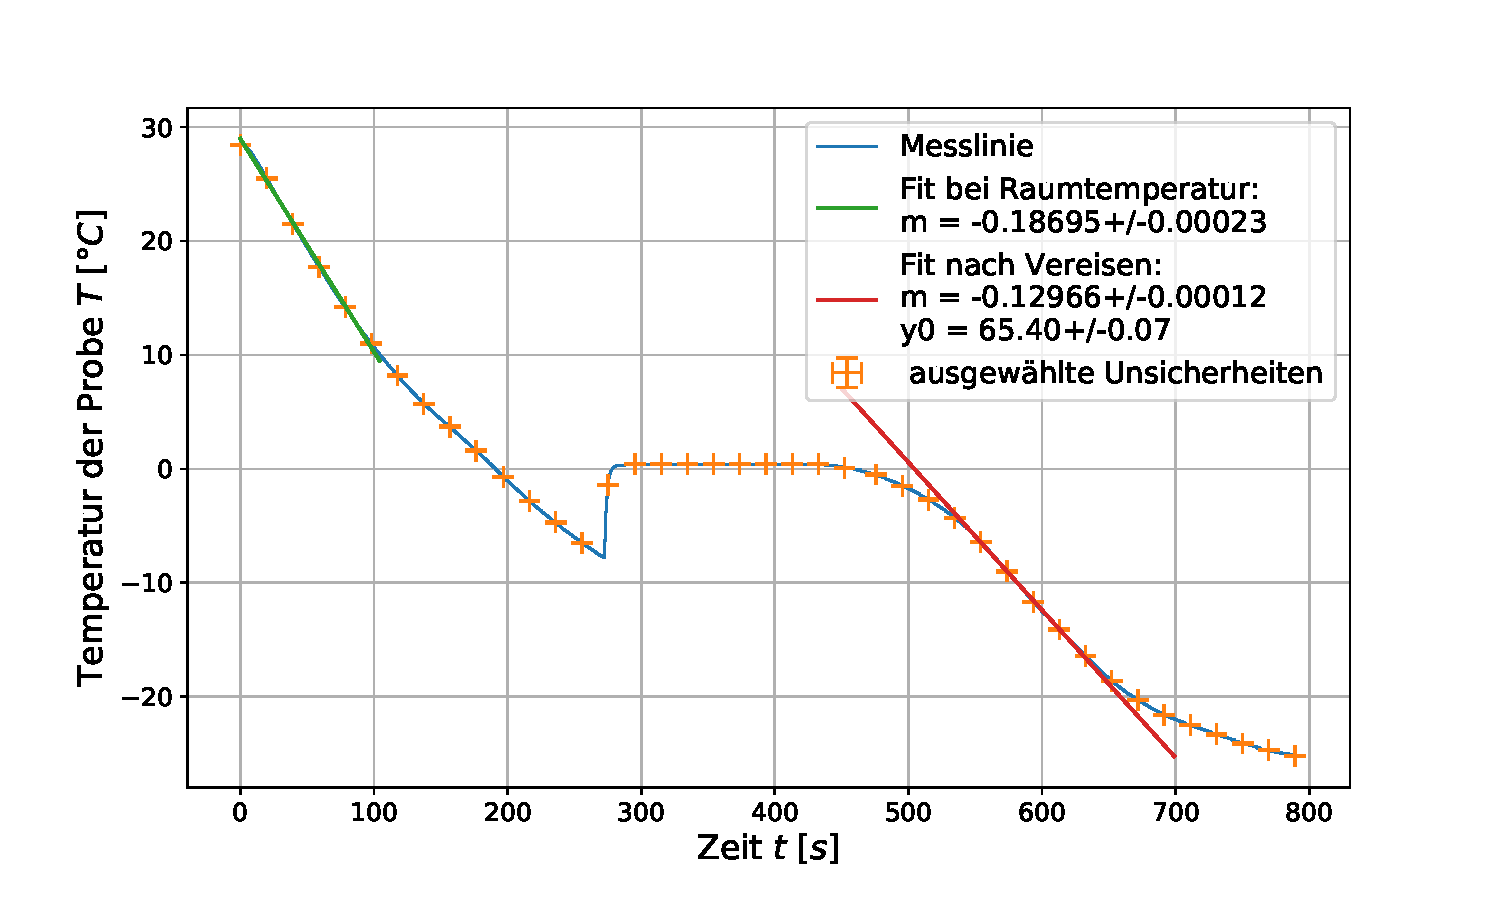
\includegraphics[width=\textwidth]{data/kalt_machen.pdf}
		\caption{Temperatur-Verlauf des Wassers bei der Kältemaschine.}
		\label{fig:Kältemaschine}	
	\end{figure}
	Nun zu der Verwendung des Motors als Kältemaschine.
	Dazu wurde der Zylinderkopf wieder verschraubt und \SI{1}{\milli\liter} destilliertes Wasser in das daran befestigte Reagenzglas gefüllt.
	Abbildung \ref{fig:Kältemaschine} zeigt den aufgenommen Verlauf der Temperatur des Wassers mit einer Abtastrate von \SI{10}{\hertz}.
	\begin{figure}[ht]
		\centering
		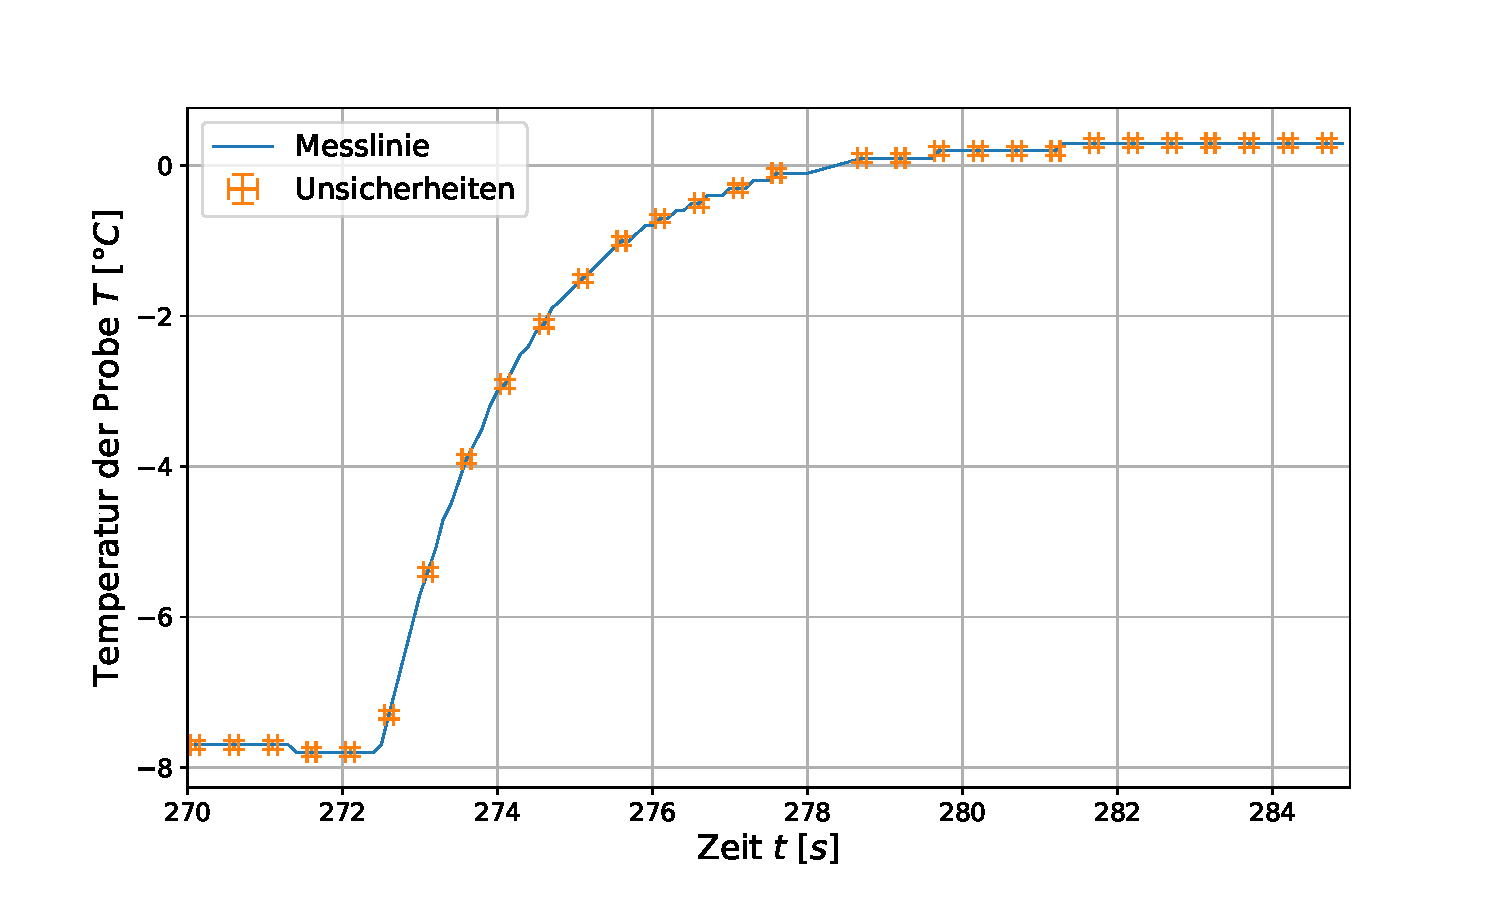
\includegraphics[width=\textwidth]{data/kalt_sprung.pdf}
		\caption{Genauere Darstellung des Sprungs in der Temperaturkurve der Kältemaschine.}
		\label{fig:KaltSprung}	
	\end{figure} 
	Auffällig daran ist der schlagartige Anstieg von ca. \SI{8}{\celsius} auf ungefähr \SI{0}{\celsius} und der darauf folgende konstante Bereich, bis die Temperatur wieder anfängt zu sinken.
	Dieser Sprung wird in Abbildung \ref{fig:KaltSprung} deutlicher dargestellt.
	Nachdem eine Temperatur von ca. \SI{-26,7}{\celsius} erreicht wurde, wurde zudem eine Messung der Temperatur des abfließenden Kühlwassers $T_\text{Abfluss} = \SI{26,6+-0,03}{\celsius}$ und der im Reservoir $T_\text{Reservoir} = \SI{25,3+-0,03}{\celsius}$ durchgeführt.
	Die Schmelzwärme des Wassers lässt sich über ... abschätzen. %TODO Rechenweg ↓ Schmelzwärme
	Für die Kühlleistung ...%TODO Rechenweg ↓ Leistung
	
	\begin{figure}[ht]
		\centering
		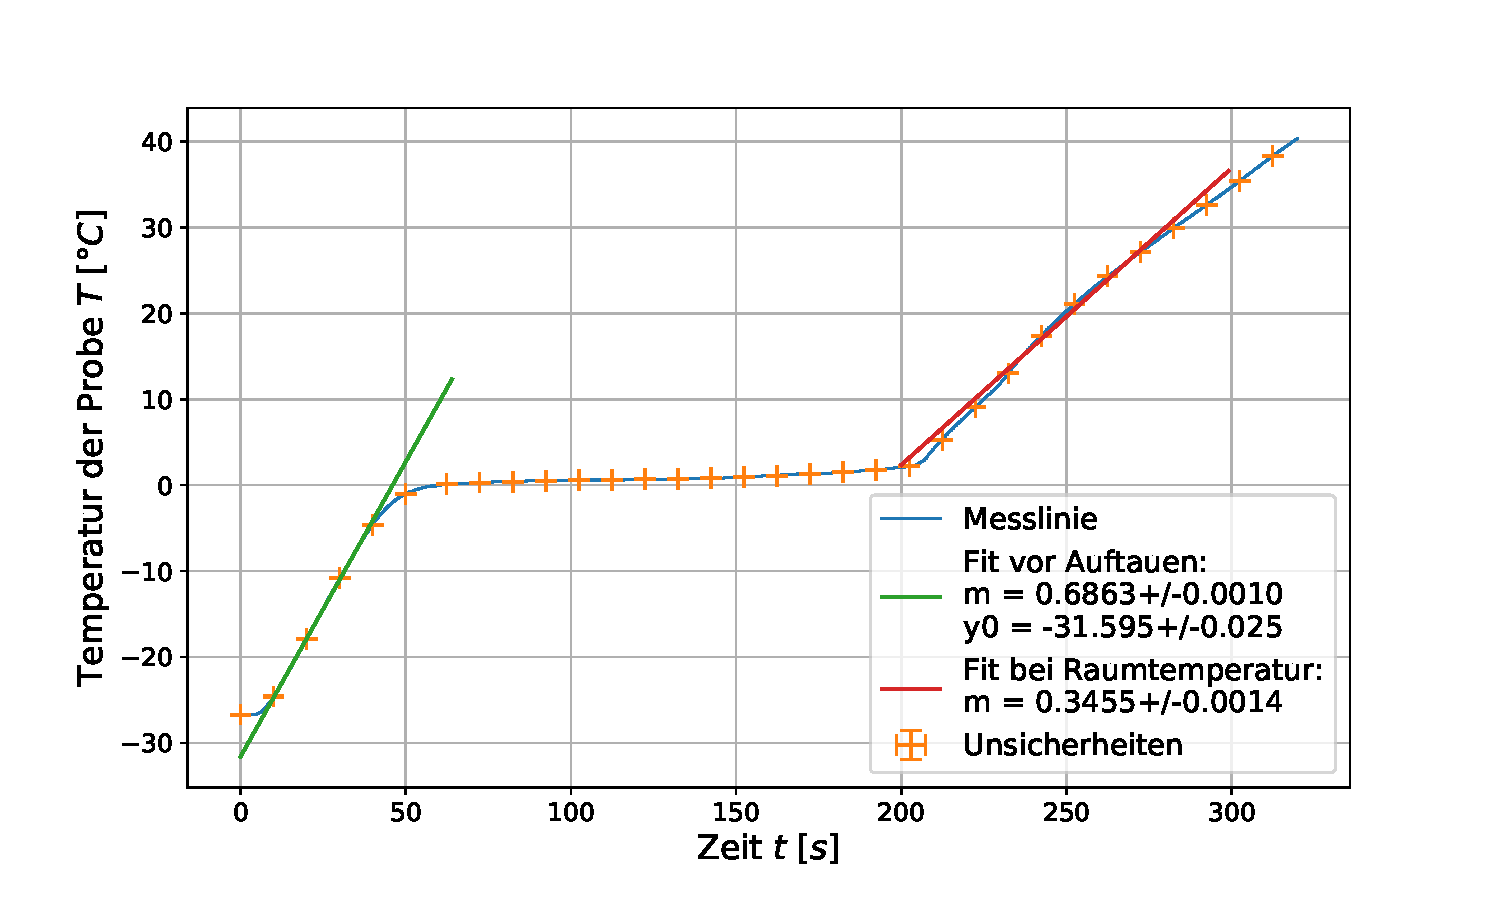
\includegraphics[width=\textwidth]{data/warm_machen.pdf}
		\caption{Temperatur-Verlauf des Wassers bei der Wärmepumpe.}
		\label{fig:Wärmepumpe}	
	\end{figure}
	Analog zur Kältemaschine verlief die Untersuchung der Wärmepumpe. 
	Die Temperatur des Wassers bei diesem Vorgang ist in Abb. \ref{fig:Wärmepumpe} aufgetragen.
	Bei dieser Kurve wurde ein ähnlicher Verlauf verzeichnet.
	Hier tritt jedoch kein Sprung auf, die Temperatur bleibt jedoch wie zuvor bei ungefähr \SI{0}{\celsius} für einige Zeit konstant, bevor sie wieder ansteigt.
	Auch hier wurde erneut eine Messung der Temperatur des abfließenden Kühlwassers $T_\text{Abfluss} = \SI{25,5+-0,03}{\celsius}$ und der im Reservoir $T_\text{Reservoir} = \SI{25,5+-0,03}{\celsius}$ durchgeführt.
	Dies geschah bei der Temperatur des Wassers von ca. \SI{40,4}{\celsius}.
	Die Berechnung der Schmelzwärme und der Heizleistung aus dieser Kurve verlaufen analog zu denen bei der Kältemaschine.
	
\section{Diskussion}
	
	Nun stellt sich die Frage, ob die Ziele der Untersuchung erreicht wurden.
	Dazu wird zunächst betrachtet, ob die Werte für Reibungsarbeit und Heiz- bzw. Kühlleistung physikalisch sinnvoll sind.
	Der ermittelte Wert für die Reibungsarbeit entspricht %TODO.
	Dieser ist %TODO
	Für Heiz- und Kühlleistung ergaben sich %TODO
	Bei diesen %TODO
	
	Der Sprung bei dem Verlauf der Temperatur und der darauffolgende konstante Bereich bei der Kältemaschine lässt sich über die SChmelzwärme erklären.
	Diese Wärme wird benötigt um von dem festen Zustand in den flüssigen zu wechseln.
	Umgekehrt wird diese Wärme freigelassen, wenn der Wechsel von flüssig nach fest stattfindet.
	Dies geschieht nicht direkt bei \SI{0}{\celsius}, sondern erst nachdem sich Kristalle in der Flüssigkeit gebildet haben, welche sich schlagartig vermehren und zu dem Gefrieren der Flüssigkeit führen.
	Bis zur kompletten Kristallisierung bleibt die Temperatur bei ungefähr \SI{0}{\celsius} und fällt danach wieder ab.
	Umgekehrt muss bei der Wärmepumpe die erforderliche Schmelzwärme dem Eis hinzu geführt werden, weswegen auch hier der Temperaturverlauf für einige Zeit konstant bleibt. 
	Dass die ermittelten Werte für die Schmelzwärme aus beiden Messungen exakt übereinstimmen ist hervorragend.
	Zudem unterscheidet sich dieser Wert um ?\% von dem Literaturwert. %TODO
	
	Bei der spezifischen Wärme von Eis wurde hier ein Wert von ... bestimmt. %TODO
	Dieser unterscheidet sich um ?\% von dem Literaturwert. %TODO